\chapter{Métodos para resolver recurrencias}

\section{El método del árbol recursivo}

El método del árbol recursivo es un método gráfico e informal para resolver recurrencias y consiste en dibujar un árbol donde cada nodo representa el tiempo requerido para resolver un subproblema.
Al sumar el valor de todos los nodos del árbol, se puede obtener la solución de la recurrencia.
Antes de estudiar el método en sí, es importante recordar algunos conceptos sobre árboles.

Sea \(k\in\mathbb{N}\), un \textbf{árbol} \(\boldsymbol{k}\)\textbf{-ario} es un árbol enraizado donde cada nodo tiene a lo más \(k\) hijos. 
Un árbol \(k\)-ario \textbf{lleno} es aquél donde cada nodo es una hoja o tiene exactamente \(k\) hijos. 
La \textbf{profundidad} de un nodo es la distancia más corta entre dicho nodo y la raíz. 
Por definición, la raíz tiene una profundidad de 0.
Un árbol \(k\)-ario \textbf{completo} es un árbol lleno donde todas las hojas tienen la misma profundidad.
En un árbol \(k\)-ario completo, el número de nodos a profundidad \(d\) está dado por \(k^d\).
La \textbf{altura} de un árbol es la profundidad más grande de todos los nodos.
Así, la altura de un árbol \(k\)-ario completo de \(n\) hojas está dado por \(\log_k{n}\).
El número de nodos internos en un árbol \(k\)-ario completo de altura \(h\) está dado por
\[
  1+k+k^2+\dots+k^{h-1} = 
  \sum_{d=0}^{h-1}k^d =
  \sum_{d=1}^{h}k^d =
  \dfrac{k^h-1}{k-1}.
\]

\newpage
El método del árbol recursivo consta de los sig. pasos:

\begin{enumerate}
  \item Se dibuja el árbol recursivo de la recurrencia cumpliendo con las sig. características:
  \begin{itemize}
    \item La raíz contiene la expresión \(f(n)\) que representa el tiempo de ejecución requerido por la división y/o la combinación.
    \item Cada nodo interno contiene la expresión \(f(n_i)\), donde \(n_i<n\) es el tamaño del subproblema \(i\).
    \item Cada hoja contiene el tiempo de ejecución requerido por el caso base, que casi siempre es \(\Theta(1)\).
    \item Cada nodo interno tiene una cantidad de hijos equivalente al número de subproblemas en que se divide la entrada de cada llamada recursiva.
  \end{itemize}
  \item Se calcula la altura del árbol; esto es, la ruta más larga que sigue el algoritmo en el árbol para llegar al caso base.
  \item Se calcula la cantidad de hojas; esto es, el número de nodos en el nivel más profundo.
  \item Se suman los valores de todos los nodos por cada nivel.
  \item Se suman los resultados de todos los niveles, obtenidos en el paso anterior.
  \item Se resuelve la expresión resultante. %para obtener la forma cerrada.
\end{enumerate}

\begin{figure*}[t]
  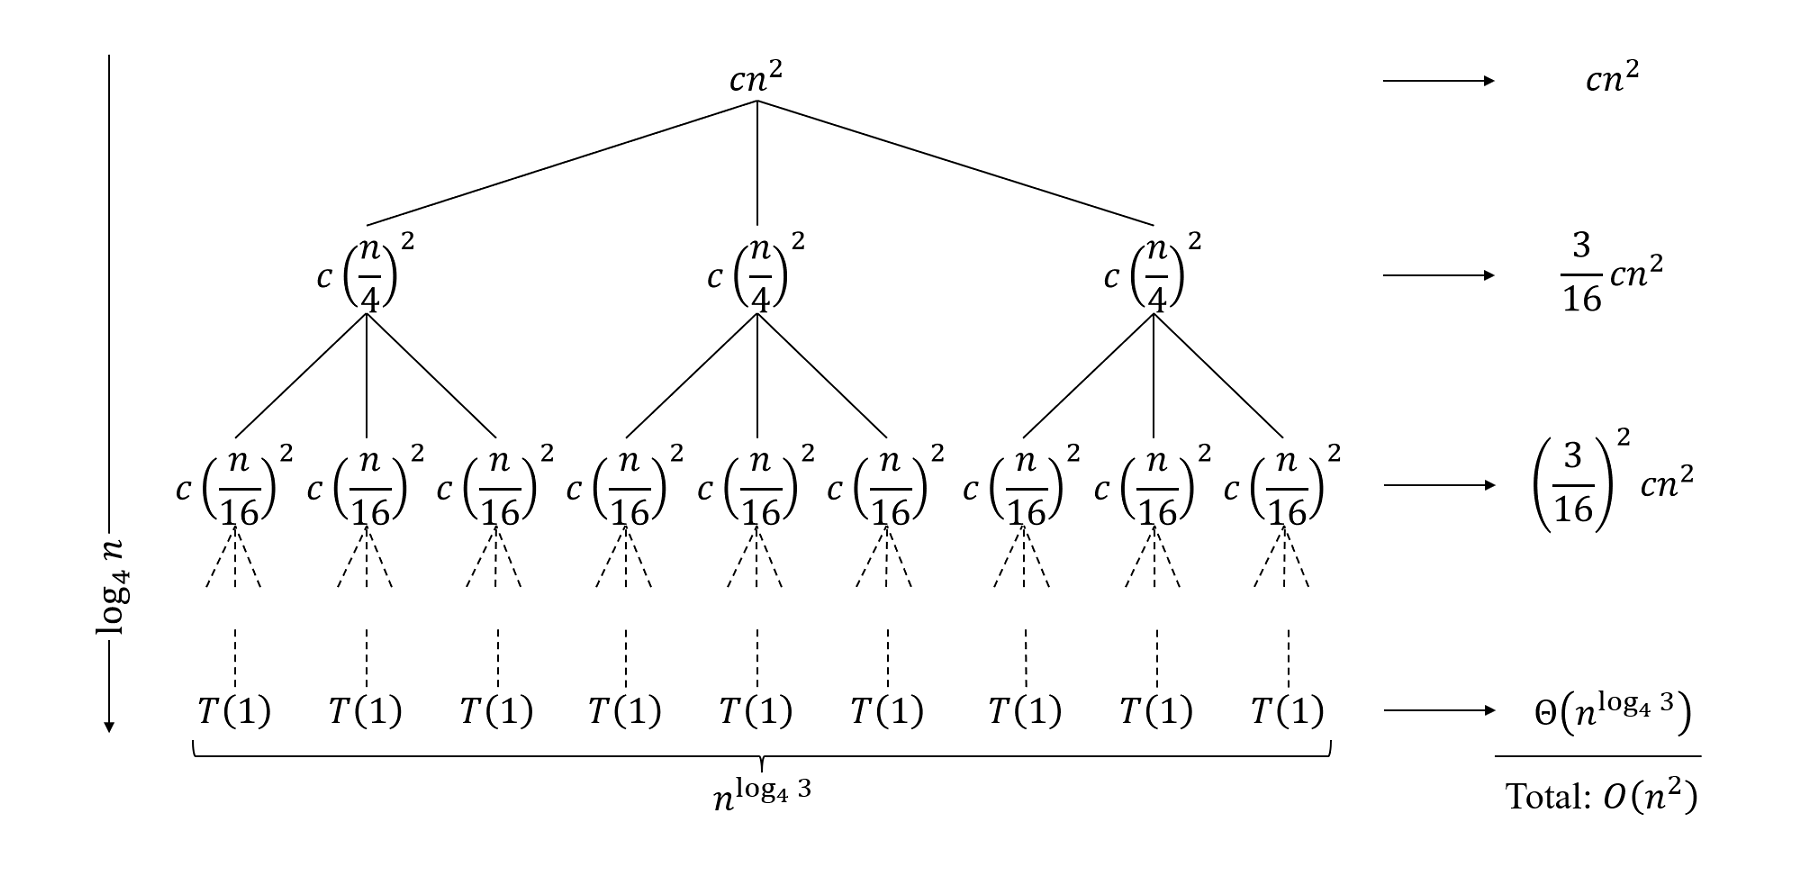
\includegraphics[width=1\textwidth]{figuras/recursion-tree.png}
  \caption{Usando el método del árbol recursivo para resolver la recurrencia \(T(n)=3T(n/4)+cn^{2}\).}
  \label{fig:recursion_tree}
\end{figure*}

\newpage

\begin{expl}
  Considérese la recurrencia \(T(n)=3T(n/4)+cn^2\). 
  Se debe dibujar el árbol recursivo, el cual se muestra en la Figura \ref{fig:recursion_tree}.
  Después, se debe calcular la altura del árbol. 
  Dado que el valor de \(n\) se reduce en un factor de \(1/4\) en cada nivel, la altura es el número de niveles que deben de recorrerse hasta llegar a 1. Así, la altura \(h\) puede calcularse como
  \[
    \begin{aligned}
      \left(\dfrac{1}{4}\right)^h\cdot n &= 1 \\
      \dfrac{1}{4^h}\cdot n &= 1 \\
      n &= 4^h \\
      \log_4{n} &= h.
    \end{aligned}
  \]
  
  Luego, se debe calcular el número de hojas.
  Dado que cada nodo tiene exactamente 3 hijos, el número de hojas está dado por
  \[
    3^h = 3^{\log_4{n}} = n^{\log_4{3}}.
  \]
  
  El siguiente paso es calcular el tiempo total de cada nivel.
  En la Figura \ref{fig:recursion_tree}, se observa que de dicha suma surge un patrón que se repite en función de \(cn^2\).
  En cuanto a la suma del último nivel, dado que el tiempo requerido por el caso base está dado por \(T(1)=\Theta(1)\), dicha suma es igual al número de hojas, que ya se calculó.
  
  Por último, se suman los tiempos de todos los niveles, lo que resulta en la sig. expresión:
  
  \begin{align*}
    T(n)&=\sum_{i=0}^{\log_{4}n-1}\left(\dfrac{3}{16}\right)^{i}\cdot cn^{2}+\Theta(n^{\log_{4}3}) \\
    &<\sum_{i=0}^{\infty}\left(\dfrac{3}{16}\right)^{i}\cdot cn^{2}+\Theta(n^{\log_{4}3}) \\
    &=\dfrac{1}{1-3/16}\cdot cn^{2}+\Theta(n^{\log_{4}3}) \\
    &=\dfrac{16}{13}\cdot cn^{2}+\Theta(n^{\log_{4}3}) \\
    &=O(n^{2})+O(n^{\log_{4}3}) \\
    &=O(n^{2}).
  \end{align*}
	\exend
\end{expl}
\newpage



\section{El método de sustitución}

El método de sustitución es un método formal que consiste en resolver una recurrencia utilizando inducción matemática. 
Específicamente, este método consta de los sig. pasos:
\begin{enumerate}
  \item Se propone una cota asintótica como la solución tentativa de la recurrencia.
  \item Se utiliza inducción para demostrar que la recurrencia cumple con la cota propuesta y para encontrar las constantes de dicha cota.
\end{enumerate}
Este método se puede utilizar para calcular tanto una cota superior como una inferior.

\paragraph{Para proponer una buena solución tentativa.}{%
  Se puede utilizar el método del árbol recursivo para obtener una solución tentativa.
  Después, se puede usar el método de sustitución para demostrar que dicha solución es correcta o para ajustar la cota en caso de que no lo sea.
  Otra alternativa es que, si la recurrencia tiene una forma similar a alguna otra cuya solución ya se conoce, se puede proponer esa solución como la solución tentativa.
  Como último recurso, se pueden proponer dos cotas holgadas, una inferior y  una superior, y ajustarlas gradualmente hasta que converjan en la solución correcta. 
}
\paragraph{Diferencias con la inducción matemática.}{%
  El caso base se demuestra hasta el final y no al principio de la demostración.
  La hipótesis inductiva consiste en suponer que la cota se cumple para cualquier subproblema, \(T(n_i)\), donde \(n_i<n\). 
  El paso inductivo consiste en sustituir \(T(n_i)\) (en la recurrencia original) por la forma exacta de la cota propuesta en la hipótesis inductiva. 
  Este paso da origen al nombre del método.
}
\paragraph{Cuidado con la notación asintótica.} {%
  El objetivo del método de sustitución es demostrar algebraicamente que 
  la cota propuesta se cumple de \emph{forma exacta}.
  Es incorrecto aplicar la notación asintótica en el paso inductivo para deshacerse de constantes o términos problemáticos.
}

\newpage
\begin{expl}
  \label{ex:recurrence_substitution}
  Considérese la recurrencia \(T(n)=2T(\lfloor n/2 \rfloor)+n\) y supóngase que se propone \(O(n\lg{n})\) como la solución tentativa. 
  Entonces, se busca demostrar que \(T(n)\leq cn\lg{n}\) para alguna constante \(c>0\).
  \begin{description}
    \item[Hipótesis inductiva] Supóngase que \(T(\lfloor n/2\rfloor)\leq c\lfloor n/2\rfloor\lg\lfloor n/2\rfloor\).
    \item[Paso inductivo] Sustituyendo la hipótesis inductiva en la recurrencia original, se tiene:
    \begin{align*}
      T(n) &\leq2c\lfloor n/2\rfloor\lg\lfloor n/2\rfloor+n \\
      &\leq cn\lg(n/2)+n \\
      &=cn\lg n-cn\lg2+n \\
      &=cn\lg{n}-cn+n \\
      &\leq cn\lg n.
    \end{align*}
    Aparentemente, la solución propuesta es la correcta (para toda \(c\geq 1\)). 
    Sin embargo, hace falta demostrar que esta solución también se cumple para la condición de paro de la recurrencia. 
    Esto debe demuestrarse por construcción; esto es, se debe encontrar un valor para \(c\) que satisfaga la cota en la condición de paro. 
    A continuación, se muestra cómo esto puede llevar a ciertos problemas. 
    \item[Caso base] Supóngase que \(T(1)=1\). 
    Aplicando la cota propuesta a la condición de paro, se tiene que \(T(1)\leq cn\lg n=c\lg{1}=0\), lo que contradice que \(T(1)=1\). 
    Por lo tanto, la solución propuesta falla en el caso base. 
    Sin embargo, hay que recordar que la definición de la notación asintótica requiere que la cota se cumpla únicamente para un valor de \(n\) mayor que algún umbral \(n_{0}\) que \emph{uno es libre de elegir a voluntad}. 
    Esto quiere decir que no es obligatorio utilizar la condición de paro de la recurrencia como el caso base de la inducción. 
    Para este ejemplo, obsérvese que \(T(\lfloor2/2\rfloor)=T(\lfloor3/2\rfloor)=T(1)\), por lo que se puede utilizar \(T(2)\) y \(T(3)\) como el caso base. 
    Esto es equivalente a elegir \(n_0=2\).
    Aplicando la hipótesis inductiva al nuevo caso base, se tiene:
    \begin{align*}
      T(2) & \leq 2c\lg2 & T(3) & \leq 3c\lg3 \\
      2T(\lfloor 2/2 \rfloor) + 2 & \leq 2c & 2T(\lfloor 3/2 \rfloor) + 3 & \leq 3c(1.585) \\
      2T(1) + 2 & \leq2c & 2T(1) + 3 & \leq 3c(1.585) \\
      4 & \leq 2c & 5 & \leq 3c(1.585) \\
      2 & \leq c, & \dfrac{5}{4.755} & \leq c.
    \end{align*}
    Por lo tanto, queda demostrado que \(T(n)\leq cn\lg{n}\) para toda \(c\geq 2\). \exend
  \end{description}
\end{expl}

\newpage
\begin{expl}
    Considérese ahora la recurrencia \(T(n)=T(\lfloor n/2\rfloor)+T(\lceil n/2\rceil)+1\) y supóngase que se propone \(O(n)\) como la solución tentativa. 
    Se busca demostrar que \(T(n)\leq cn\) para alguna \(c>0\).
    \begin{description}
      \item[Hipótesis inductiva] Supóngase que \(T(\lfloor n/2\rfloor)\leq c\lfloor n/2\rfloor\) y que \(T(\lceil n/2\rceil)\leq c\lceil n/2\rceil\).
      \item[Paso inductivo] Sustituyendo la hipótesis inductiva en la recurrencia original, se tiene: \(T(n) \leq c\lfloor n/2 \rfloor + 1 = cn + 1\).
      Esto sugiere que la solución propuesta no es correcta.
      En este ejemplo, se ve que el término \(+1\) impide que la igualdad se cumpla de forma exacta.
      En lugar de proponer una cota más holgada, se propone une nueva hipótesis inductiva.
      \item[Nueva H.I.] Supóngase que \(T(\lfloor n/2\rfloor)\leq c\lfloor n/2\rfloor-d\) y que \(T(\lceil n/2\rceil)\leq c\lceil n/2\rceil-d\), donde \(d\in\mathbb{R}\) tal que \(d\geq 0\).
      \item[Paso inductivo] Sustituyendo la hipótesis inductiva en la recurrencia original, se tiene lo sig.:
      \begin{align*}
        T(n) &\leq c\lfloor n/2\rfloor-d+c\lceil n/2\rceil-d+1\\
        &=cn-2d+1\\
        &\leq cn-d.
      \end{align*}
      Esto se cumple para toda \(d\geq 1\). 
      Ahora solo queda demostrar que la cota se cumple para la condición de paro.
      \item[Caso base] Obsérvese que \(n=2\) es el valor más pequeño que resulta en \(T(1)\), tanto para \(T(\lfloor n/2 \rfloor)\) como para \(T(\lceil n/2 \rceil)\). 
      Aplicando la hipótesis inductiva a estos términos, se tiene que:
      \begin{align*}
        T(2) &\leq 2c-d\\
        T(\lfloor 2/2 \rfloor) + T(\lceil 2/2 \rceil) + 1 &\leq 2c-d \\
        2T(1) + 1 &\leq 2c - d \\
        \dfrac{2T(1)+1+d}{2} &\leq c \\
        T(1) + \dfrac{1+d}{2} &\leq c.
      \end{align*}
      \exend
    \end{description}
\end{expl}


\newpage
\section{El Teorema Maestro}

\begin{thm}[\textbf{Teorema Maestro}]
  Sean \(a,b,n\in\mathbb{N}\), donde \(a\) y \(b\) son constantes y \(b>1\), sea \(f:\mathbb{N}\to\mathbb{N}\) una función asintóticamente positiva y sea \(c=\log_{b}a\). 
  La recurrencia \(T(n)=aT(n/b)+f(n)\) puede resolverse aplicando uno de los sig. casos:
  \begin{enumerate}
    \item Si \(f(n)=O(n^{c-\varepsilon})\) para alguna constante real $\varepsilon>0$, entonces \(T(n)=\Theta(n^{c})\).
    \item Si \(f(n)=\Theta(n^c)\), entonces \(T(n)=\Theta(n^{c}\log{n})\).
    \item Si \(f(n)=\Omega(n^{c+\varepsilon})\) y si, además, \(af(n/b)\leq kf(n)\) para alguna constante real \(k<1\) y para todo valor de \(n\) mayor que algún umbral, entonces \(T=\Theta(f)\).
  \end{enumerate}
\end{thm}

\begin{rem}
  En el Teorema Maestro, el término \(n/b\) de la recurrencia \(T(n)\) también puede interpretarse como \(\lceil n/b\rceil\) o \(\lfloor n/b\rfloor\).
\end{rem}

El Torema Maestro solo puede aplicarse a recurrencias que dividen el problema en \(a\) subproblemas \emph{del mismo tamaño}, y donde, en cada subproblema, el tamaño de la entrada se reduce en un factor de \(1/b\).
La función \(f(n)\) representa el tiempo de ejecución para dividir el problema y/o combinar las soluciones parciales de los subproblemas.
La función \(n^c\) representa el número de hojas en el árbol recursivo de la recurrencia.

Intuitivamente, el Teorema Maestro indica que, comparando \(n^c\) con \(f(n)\), la función que crece más rápido es la solución de la recurrencia.
\begin{itemize}
  \item \textit{Caso 1}: \(n^c\) crece más rápido; esto es, el tiempo requerido para resolver cada subproblema eventualmente supera el tiempo requerido por la división y/o combinación.
  \item \textit{Caso 2}: ambas funciones, \(f(n)\) y \(n^c\), tienen la misma tasa de crecimiento.
  En este caso, la solución es el orden de crecimiento de estas funciones, multiplicado por un factor logarítmico que representa la altura del árbol recursivo (ya que cada nivel del árbol requiere el mismo tiempo de ejecución).
  \item \textit{Caso 3}: \(f(n)\) crece más rápido que \(n^c\). 
  Si \(f(n)\), además, cumple con la \textbf{condición de regularidad}, entonces esta función es la solución de la recurrencia.
\end{itemize}

\section{Notas bibliográficas}

En el libro de \textcite{cormen_2009}, págs. 97-106, se proporciona la demostración del Teorema Maestro.
Además, en las págs. 112-113, se describe el \textbf{método de Akra-Bazzi} \citep{akra_1998,leighton_1996}, que se utiliza para resolver recurrencias donde el problema se divide en subproblemas que difieren mucho de tamaño.
Este método trabaja con variables contínuas.
Por otro lado, \textcite{drmota_2013} presentan una especialización del método de Akra-Bazzi que trabaja con variables discretas. 

\marginnote[-1\baselineskip]{%
  \textbf{Literatura consultada}: \textcite{cormen_2009} pp. 65-67, 83-97.
}
